\section{Structural Breaks and Chow Test}

In this section, we employ the Chow test to assess whether a significant structural change occurs in the regression models at 
specific points in time. 
To ensure the robustness of our analysis, we first established a minimum data subset size for the unrestricted models, 
setting it to 10\% of the total dataset, in order to maintain statistical validity while preserving sufficient data for
meaningful comparisons.
Subsequently, the Chow test was systematically applied to all linear regressions conducted on the selected equities, 
allowing us to identify potential structural breaks across the dataset, that is, significant changes in the regression
parameters caused by external shocks, market-wide events, or company-specific factors. 
These structural breaks may reflect shifts in the relationship between excess returns and market behaviour, such as changes in
systematic risk $(\beta)$ or the presence of unexplained excess returns $(\alpha)$ due to macroeconomic conditions, regulatory 
adjustments or sector-specific developments.
To identify these structural breaks, we analyzed the p-values obtained from the Chow test for each equity over time: 
a p-value below the threshold of 0.01 was interpreted as evidence of a structural break at that particular point in time,
signaling that the CAPM parameters had changed significantly.
In this analysis, only periods of at least two consecutive months with p-values below the threshold were considered as
break dates, ensuring that the identified breaks reflect sustained shifts rather than noise or transient fluctuations.

\begin{figure}[h!]
    \centering
    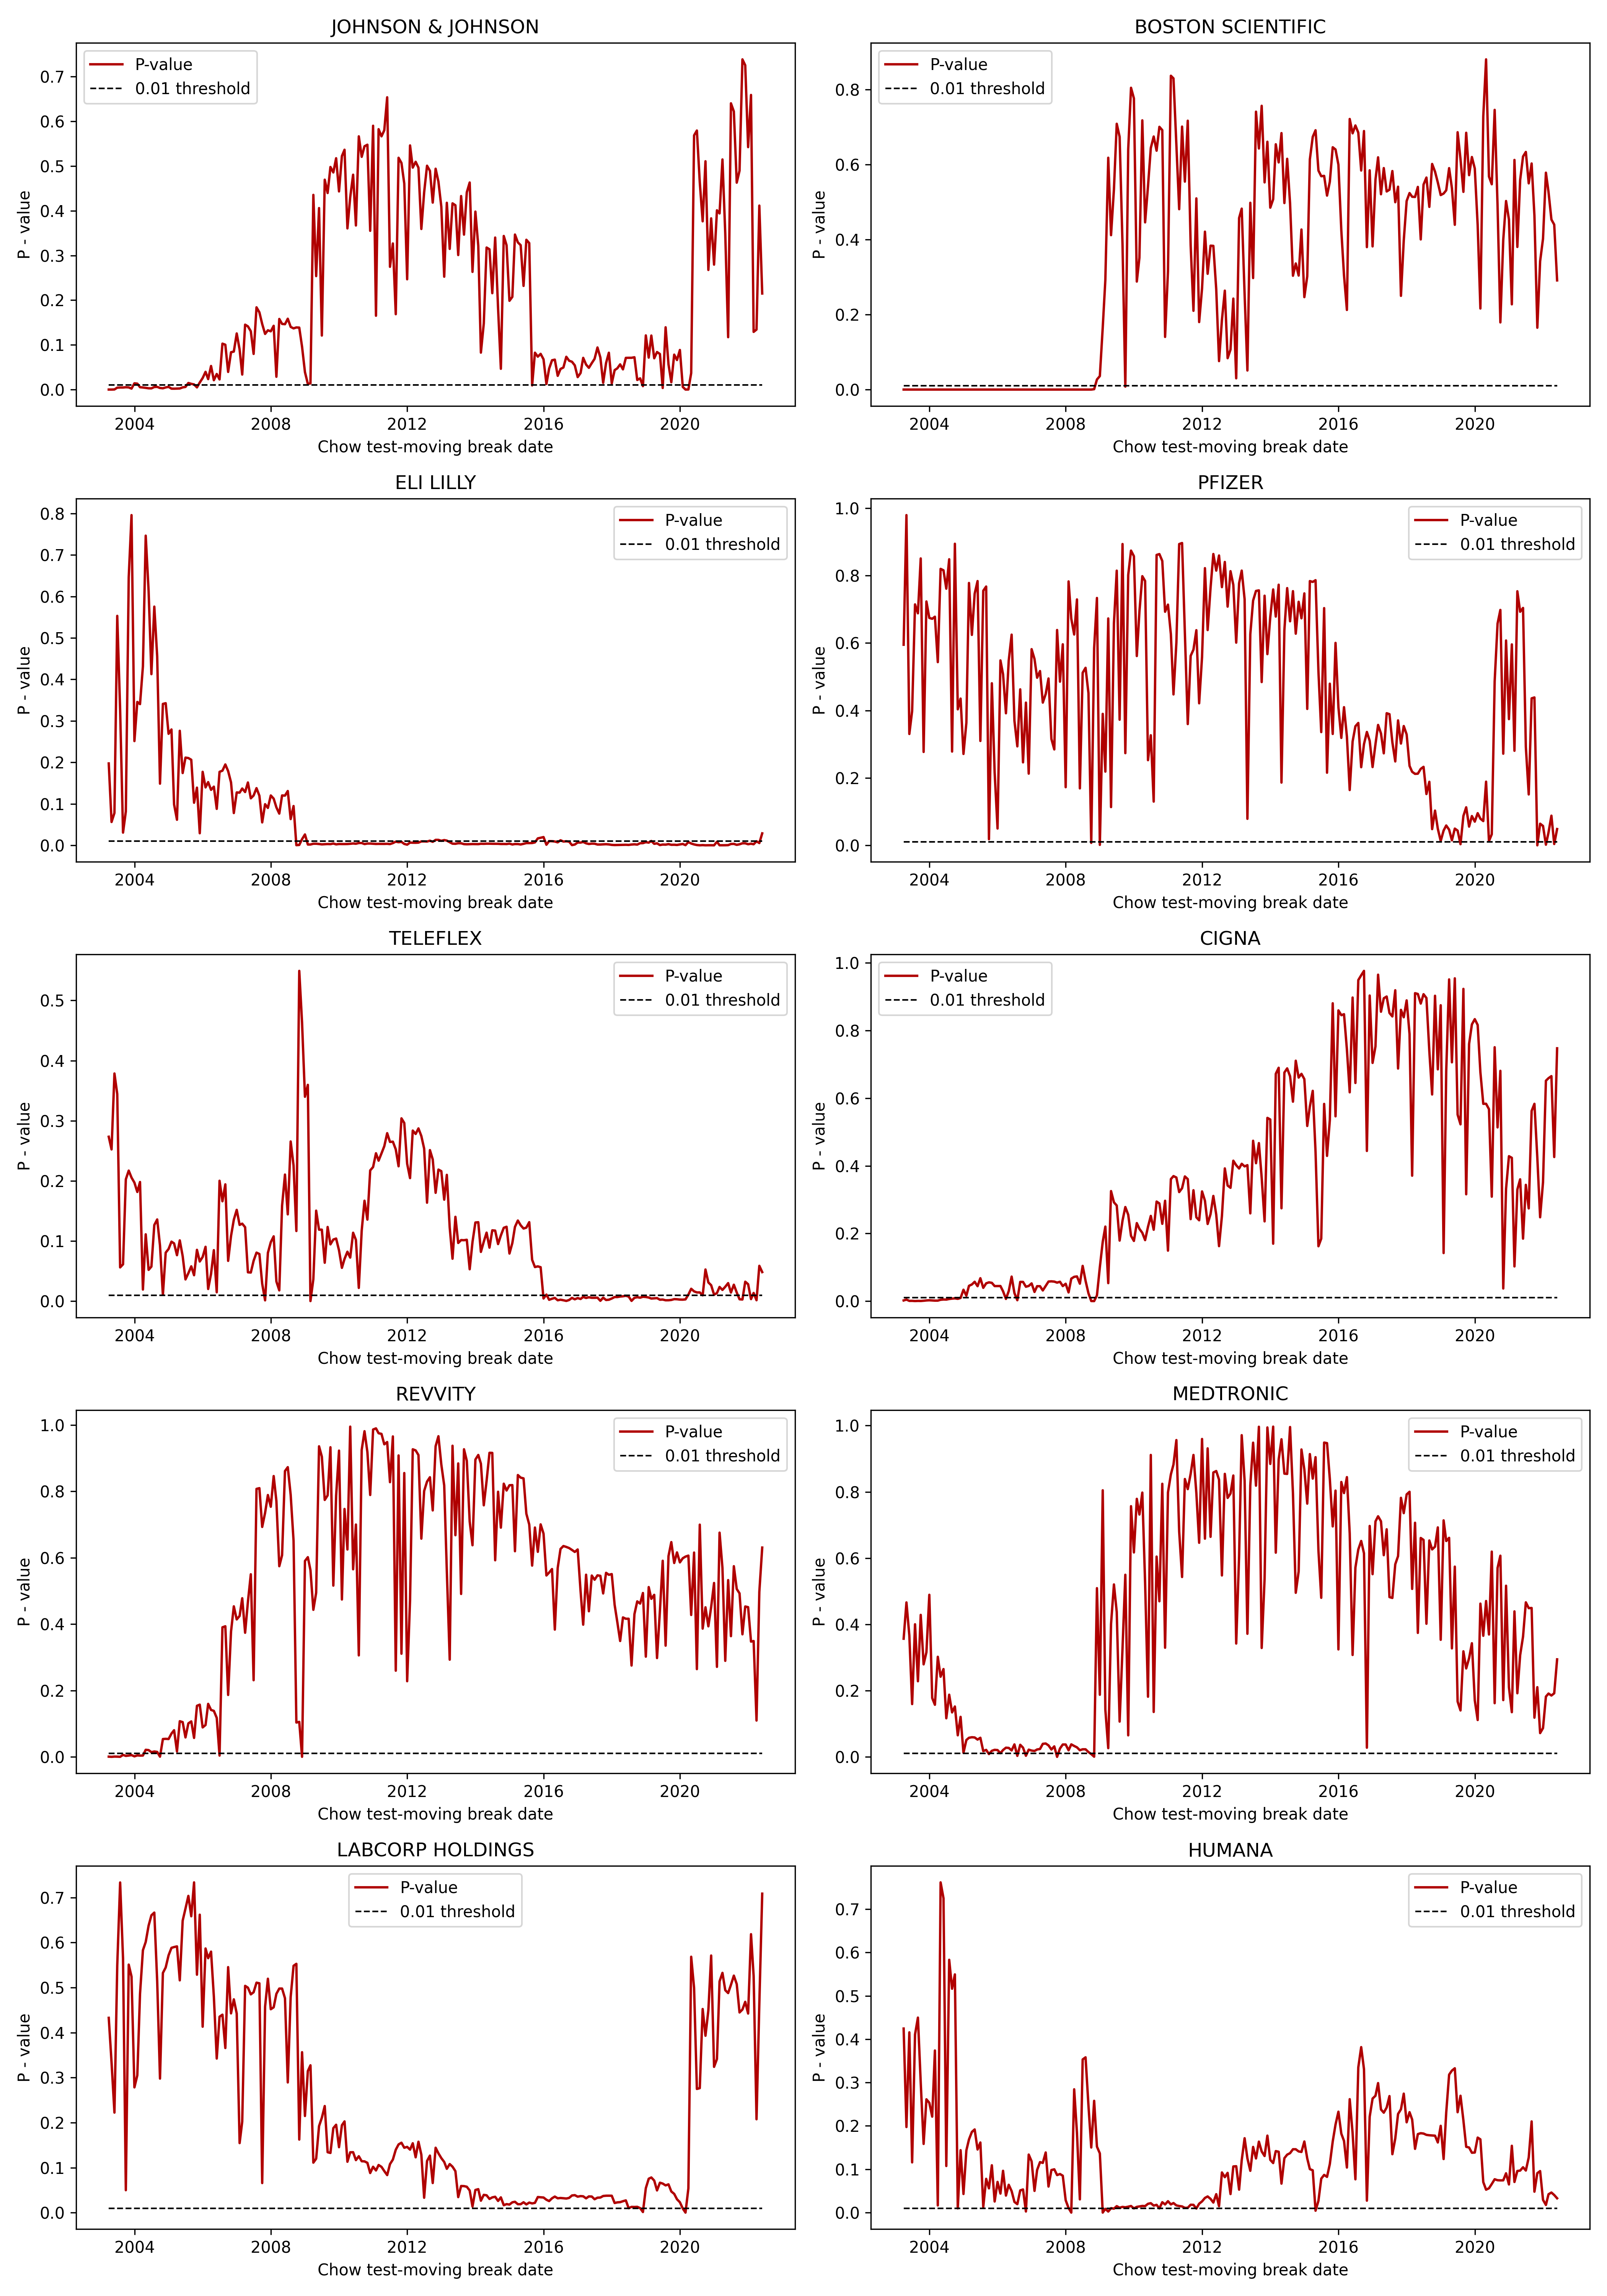
\includegraphics[width=0.8\textwidth]{images/chowmoving.png}
    \caption{Chow Test performed for all equities in search of structural breaks.}\label{fig:chowmoving}
\end{figure}

The results of this analysis are displayed in Figure~\ref{fig:chowmoving}, highlighting that different equities exhibit 
fundamentally distinct behaviors. 
Notably, certain equities, such as \textit{Eli Lilly}, \textit{Boston Scientific}, and \textit{Teleflex}, show p-values
consistently below the 0.01 threshold for extended periods, indicating prolonged structural breaks; this raises the question
of whether the CAPM relationship for these equities in these periods is truly linear or whether a different modeling approach
may be warranted.

\section{Periods of Shared Structural Breaks}

Despite these observations, no clear or consistent pattern of structural breaks emerges across all equities; to explore 
potential commonalities further, an additional histogram was generated (Figure~\ref{fig:struct_break_freqs}), which illustrates
the frequency and overlap of structural breaks shared among different equities.

\begin{figure}[h!]
    \centering
    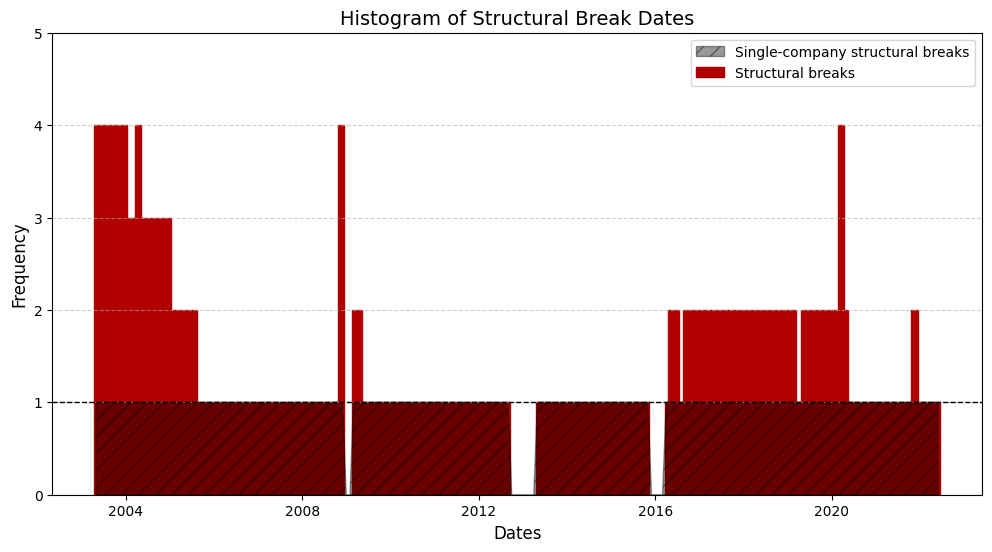
\includegraphics[width=0.8\textwidth]{images/struct_break_freqs.png}
    \caption{Frequency of months identified as structural break points.}\label{fig:struct_break_freqs}
\end{figure}

Figure~\ref{fig:struct_break_freqs} highlights two important aspects of the data: 
first, there is no single period that constitutes a break date for all equities; the maximum number of companies sharing a 
structural break at any given time is in fact 4. 
Nonetheless, the break dates identified as significant changes to the regression parameters align closely with expectations,
in fact the data reveal break dates significantly relevant in three distinct periods of time:
\begin{itemize}
    \item  \textbf{2003}: Structural breaks are observed throughout most of the year, coinciding with the SARS epidemic. 
    This period also aligns with economic and legislative developments, including the introduction of the Medicare
    Modernization Act, which reshaped healthcare policy and access in the United States.
    \item \textbf{October and November 2008}: These months mark the onset of the 2008/2009 financial crisis.
    \item \textbf{February and March 2020}: Structural breaks during this time correspond to the emergence of the COVID-19
    pandemic and the widespread implementation of precautionary measures.
\end{itemize}

An important observation is that the structural breaks identified in 2003 extended over a prolonged period, spanning multiple
consecutive months, whereas the impact of the COVID-19 pandemic appears to have been more concentrated and shorter in duration.
The prolonged effect in 2003 could reflect the gradual adjustment of the healthcare market to the SARS epidemic and concurrent
economic and legislative changes.
In contrast, the shorter duration of structural breaks during COVID-19 may suggest that lessons learned from the SARS outbreak,
including the implementation of precautionary measures and improved epidemic preparedness, helped mitigate the impact of
subsequent epidemics on the healthcare market.
Alternatively, the healthcare market may have simply grown so significantly in size and diversification over time that it 
developed a level of resilience that enables it to absorb and adapt to substantial disruptions in the economic landscape.
This growth, coupled with advancements in technology, expanded infrastructure, and more robust financial mechanisms,
might have contributed to the market's ability to withstand even major shocks, such as those caused by the 2008 crisis and
the COVID-19 pandemic.
This explanation also accounts for the observation that the majority of equities were not significantly impacted during these
events: the increased resilience and diversification of the healthcare market may have allowed many companies to maintain
stability despite the broader economic disruptions.

\section{Chow Test on Portfolio}

In order to further investigate the impact of significant events in the economic environment, the same Chow test was 
performed on the excess returns of the portfolio. 
This approach aggregates the behavior of individual equities into a single measure, allowing for the identification of 
systemic disruptions across the healthcare market.

\begin{figure}[h!]
    \centering
    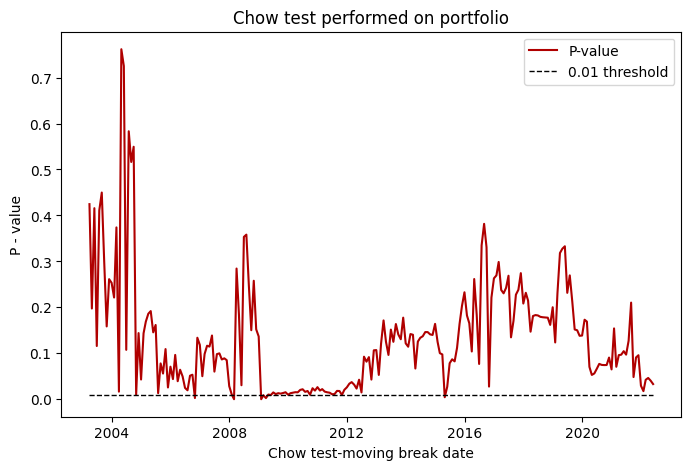
\includegraphics[width=0.8\textwidth]{images/portchowlio.png}
    \caption{Frequency of months identified as structural break points.}\label{fig:portchowlio}
\end{figure}

The results, displayed in Figure~\ref{fig:portchowlio}, reveal that there is only one time period in which structural breaks 
in the portfolio's return dynamics are particularly significant: that is the beginning of 2009, likely reflecting the
aftermath of the 2008 financial crisis.
